\documentclass[]{article}
\usepackage{lmodern}
\usepackage{amssymb,amsmath}
\usepackage{ifxetex,ifluatex}
\usepackage{fixltx2e} % provides \textsubscript
\ifnum 0\ifxetex 1\fi\ifluatex 1\fi=0 % if pdftex
  \usepackage[T1]{fontenc}
  \usepackage[utf8]{inputenc}
\else % if luatex or xelatex
  \ifxetex
    \usepackage{mathspec}
  \else
    \usepackage{fontspec}
  \fi
  \defaultfontfeatures{Ligatures=TeX,Scale=MatchLowercase}
\fi
% use upquote if available, for straight quotes in verbatim environments
\IfFileExists{upquote.sty}{\usepackage{upquote}}{}
% use microtype if available
\IfFileExists{microtype.sty}{%
\usepackage{microtype}
\UseMicrotypeSet[protrusion]{basicmath} % disable protrusion for tt fonts
}{}
\usepackage[margin=1in]{geometry}
\usepackage{hyperref}
\hypersetup{unicode=true,
            pdftitle={Effects of MPA designation and fishing pressure on the California spiny lobster (Panulirus interruptus)},
            pdfauthor={Joanna Tang, Michelle Lee, \& Rachel Behm},
            pdfborder={0 0 0},
            breaklinks=true}
\urlstyle{same}  % don't use monospace font for urls
\usepackage{graphicx,grffile}
\makeatletter
\def\maxwidth{\ifdim\Gin@nat@width>\linewidth\linewidth\else\Gin@nat@width\fi}
\def\maxheight{\ifdim\Gin@nat@height>\textheight\textheight\else\Gin@nat@height\fi}
\makeatother
% Scale images if necessary, so that they will not overflow the page
% margins by default, and it is still possible to overwrite the defaults
% using explicit options in \includegraphics[width, height, ...]{}
\setkeys{Gin}{width=\maxwidth,height=\maxheight,keepaspectratio}
\IfFileExists{parskip.sty}{%
\usepackage{parskip}
}{% else
\setlength{\parindent}{0pt}
\setlength{\parskip}{6pt plus 2pt minus 1pt}
}
\setlength{\emergencystretch}{3em}  % prevent overfull lines
\providecommand{\tightlist}{%
  \setlength{\itemsep}{0pt}\setlength{\parskip}{0pt}}
\setcounter{secnumdepth}{0}
% Redefines (sub)paragraphs to behave more like sections
\ifx\paragraph\undefined\else
\let\oldparagraph\paragraph
\renewcommand{\paragraph}[1]{\oldparagraph{#1}\mbox{}}
\fi
\ifx\subparagraph\undefined\else
\let\oldsubparagraph\subparagraph
\renewcommand{\subparagraph}[1]{\oldsubparagraph{#1}\mbox{}}
\fi

%%% Use protect on footnotes to avoid problems with footnotes in titles
\let\rmarkdownfootnote\footnote%
\def\footnote{\protect\rmarkdownfootnote}

%%% Change title format to be more compact
\usepackage{titling}

% Create subtitle command for use in maketitle
\newcommand{\subtitle}[1]{
  \posttitle{
    \begin{center}\large#1\end{center}
    }
}

\setlength{\droptitle}{-2em}

  \title{Effects of MPA designation and fishing pressure on the California spiny
lobster (\emph{Panulirus interruptus})}
    \pretitle{\vspace{\droptitle}\centering\huge}
  \posttitle{\par}
    \author{Joanna Tang, Michelle Lee, \& Rachel Behm}
    \preauthor{\centering\large\emph}
  \postauthor{\par}
      \predate{\centering\large\emph}
  \postdate{\par}
    \date{19 November 2018}

\usepackage{booktabs}
\usepackage{longtable}
\usepackage{array}
\usepackage{multirow}
\usepackage[table]{xcolor}
\usepackage{wrapfig}
\usepackage{float}
\usepackage{colortbl}
\usepackage{pdflscape}
\usepackage{tabu}
\usepackage{threeparttable}
\usepackage{threeparttablex}
\usepackage[normalem]{ulem}
\usepackage{makecell}

\begin{document}
\maketitle

\centering
\raggedright
\newpage

\section{INTRODUCTION}\label{introduction}

The California spiny lobster (\emph{Panulirus interruptus}) is one of
the most commercially and economically important lobsters in their
native range off the American West Coast\textsuperscript{1}. The
California Department of Fish and Wildlife (CDFW) estimate that nearly
600,000 individual spiny lobsters were harvested (both recreational and
commercial) in the first half of the 2008-2009
season\textsuperscript{2}. This number is, on average, half the total
harvest from Mexico\textsuperscript{3}. Given their economic importance,
there are heavy restrictions on the fish season by both the CDFW and the
Mexican government, with set harvest season dates, catch limits, and
size restrictions (greater than 82.5-82.6 mm). Moreover, in 2012, Marine
Protected Area (MPA) sites were established off the coast of
California--excluding fishing activity for the protection of natural and
cultural resources. These restrictions insure the sustainability of the
fishery and the health of the kelp forest ecosystem in which they live
and provide a unique opportunity to understand the direct impacts on
spiny lobster populations.

While the California spiny lobster remains an important fishery, the
species also plays an integral part in the marine communities of the
giant kelp forest. \emph{P. interruptus} is not only an important food
source for many predatory species such as the California sheephead,
giant sea bass, cabezone, and several species of shark, but it is also a
vital predator of sea urchins, clams, muscles, and worms. Given their
important role in maintaining ecosystem balance in the kelp forests off
the Pacific coast, understanding the human impacts on this species will
allow us to better predict the health of these kelp forest ecosystems.

MPAs, like those off the coast of California, have been established
across the United States marine areas in order to protect ecosystems,
preserve cultural resources, and sustain fishery
populations\textsuperscript{4}. Studies have shown that the
implementation of these protected areas have consistently increased the
biomass of fished species both inside and outside of MPAs, indicating
that these sites, overall, have improved the robustness and health of
marine organisms\textsuperscript{5}. For many fished species, like the
spiny lobster, these biomass increases have important implications for
the health and reproductive success as species typically reach sexual
maturity with at a certain size. Thus, understanding the direct impacts
of MPAs on spiny lobster abundance and size in relation to fishing
pressure will allow us to foreshadow the future of the species and the
ecosystems where they live.

Here we will compare California spiny lobster catch and size in the
Santa Barbara Channel from 2012 to 2017 to better understand how MPAs
affect the species and the giant kelp ecosystem. These data were
collected by the Santa Barbara Coast Long Term Ecological Research
Program (SBC LTER) as an ongoing effort to monitor the impacts of
management on marine habitats.

\section{METHODS}\label{methods}

\subsection{\texorpdfstring{\emph{Data
Collection}}{Data Collection}}\label{data-collection}

Lobster size, abundance, and fishing pressure of \emph{P. interruptus}
were collected from 2012-2017 at five SBC LTER Sites off the mainland
coast of the Santa Barbara Channel: Arroyo Quemado (AQUE), Naples Reef
(NAPL), Mohawk Reef (MOHK), Isla Vista (IVEE), and Carpinteria (CARP).
Two of the sites (NAPL and IVEE) are located in or near CDFW MPAs, while
the other three (AQUE, MOHK, and CARP) are not. Abundance and size data
were collected annually by divers in the late summer before the start of
the fishing season. Fishing pressure was determined by counting the
number of commerical trap floats. Data were collected every two to four
weeks during the lobster fishing season (October to
March)\textsuperscript{6}.

\subsection{\texorpdfstring{\emph{Statistical
Analyses}}{Statistical Analyses}}\label{statistical-analyses}

All statistical analyses and figures were created in R (version 3.4.2).

\emph{Lobster size across sites} To compare lobster size across sites,
we used lobster size data collected from all sites for 2017. We then
conducted an ANOVA test and a post-hoc Tukey's HSD test to find
differences among sites.

\emph{The affect of MPA status} To compare lobster sizes between MPA and
non-MPA sites, we used size data from 2012 and 2017. First, we tested
for normality of data across all sites. For sites with normally
distributed data, we tested for equal variances using Levene's test. We
then proceeded with two-sample, two-tailed t-tests. For sites with
non-normally distributed data, we used two-sampled, two-tailed
Mann-Whitney U tests.

\emph{Proportion of ``legal'' lobsters across sites} In order to test
for the proportion of legal-sized lobsters (carapace length over 82.6
mm) at all sites in 2017, we conducted an ANOVA test, using lobster size
data.

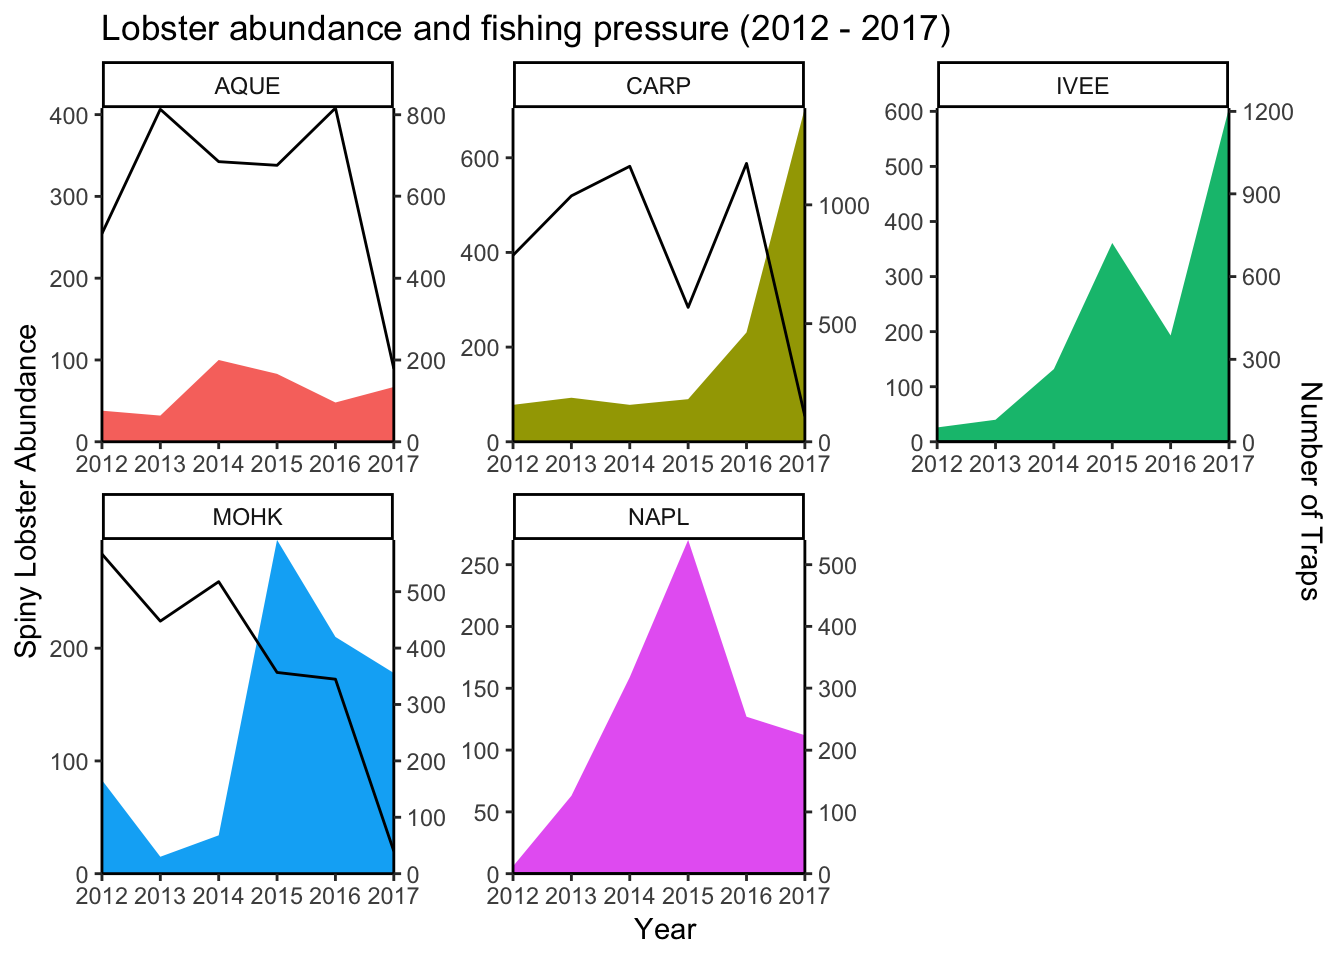
\includegraphics{assignment4_files/figure-latex/unnamed-chunk-3-1.pdf}

Overall, spiny lobster abundance has increased at all sites from 2012 to
2017. At the non-MPA sites (AQUE, CARP, MOHK) fishing pressure has
decreased from 2012 to 2017. All sites besides CARP experienced a
decrease in spiny lobster abundance in 2015. Fishing pressure and spiny
lobster abundance are inversely proportional, the abundance never
increased with fishing pressure. At site AQUE, spiny lobster abundance
has stayed relatively low from 2012 to 2017, with a slight increase
during 2013. Fishing pressure at this site remained relatively high
until 2016 where there is a steep drop off. At site CARP, spiny lobster
abundance also stayed relatively low until 2015 where it started to
drastically increase and continued to do so through 2016. Fishing
pressure at this site was high until a massive decrease in 2016. At site
MOHK, spiny lobster abundance decreased in 2012, slightly increased in
2013, massively increased in 2014, and then began slightly decreasing
from 2015 to 2017. At the MPA site IVEE, spiny lobster abundance started
low in 2012 then increased through 2014, with a drop in 2015, then a
drastic rise through 2016. At the MPA site NAPL, spiny lobster abundance
steadily grew from 2012 through 2014, with a drop in 2015, and then
stabilized through 2016.

Surprisingly, there aren't overarching trends that show an association
between MPA designation and lobster population abundance. Thus, there is
an underlying driver of population abundances other than fishing
pressure and MPA designation alone.

\includegraphics{assignment4_files/figure-latex/unnamed-chunk-4-1.pdf}

Mean lobster size (mm) in 2017 across all five sites (n(AQUE) = 67;
n(CARP) = 705; n(IVEE) = 606; n(MOHK) = 178; n(NAPL) = 112) are normally
distributed. From our ANOVA, we found that mean lobster size (mm) across
sites differ significantly (F (4, 1163) = 3.42, \emph{p} = 0.01,
\(\alpha\) = 0.05).

After performing a post-hoc Tukey's HSD test, we conclude that mean
lobster size at NAPL differs significantly from CARP (diff = 4.00 mm,
\emph{p} = 0.02), Isla Vista (diff = 4.78 mm, \emph{p} \textless{}
0.01). MOHK was fairly different when compared to NAPL, but was not
statistically significant (diff = 4.23 mm, \emph{p} = 0.06). NAPL also
had the greatest mean lobster size (76.23 mm), suggesting that the
lobster population at NAPL is the most robust or healthy. Largely, these
differences do not appear to be biologically significant as it
represents less than 6\% of the total carapace size for a theoretical
individual.

As we saw with Figure 1, we did not see any underlying trend of MPA
designation as a predictor of lobster carapace length (mm).
Interestingly, we found the largest difference in carapace length and
the largest associated p-value was between the two MPA sites (IVEE and
NAPL).

\includegraphics{assignment4_files/figure-latex/unnamed-chunk-6-1.pdf}

We found that lobster sizes across sites between 2012 and 2017 were
fairly normally distributed. Thus, we proceeded with two-sample,
two-tailed t-tests to compare lobster sizes between the two sampling
years. This test was repeated across all sites.

Between MPA sites There is no consistency between both IVEE and NAPL,
the two MPA sites, on lobster size differences between 2012 and 2017.
Isla Vista had showed a significant difference in lobster mean sizes
between 2012 and 2017 (t (28.09) = -2.20, \emph{p} = 0.04, \(\alpha\) =
0.05). NAPL, on the other hand, showed no difference in size between
years (t (5.52) = -0.66, \emph{p} = 0.54, \(\alpha\) = 0.05).

Between non-MPA sites Similar to the MPA sites, there is no consistency
between AQUE, MOHK, and CARP, the non-MPA sites, on lobster size
differences between 2012 and 2017. AQUE showed no significant difference
in lobster mean sizes between 2012 and 2017 (t (87.35) = -1.32, \emph{p}
= 0.19, \(\alpha\) = 0.05). CARP similarly showed no significant
difference in lobster mean sizes (t (91.46) = 1.23, \emph{p} = 0.22,
\(\alpha\) = 0.05). MOHK, on the other hand, showed a significant
difference in size between years (t (142.79) = 3.89, \emph{p}
\textless{} 0.01, \(\alpha\) = 0.05).

The two sites with significant differences in carapace length were NAPL,
an MPA site, and MOHK, a non-MPA site.

\includegraphics{assignment4_files/figure-latex/unnamed-chunk-9-1.pdf}

We found proportions of ``legal'' sized lobsters in catch across sites
in 2017 to be significantly different (\(\chi\)\textsuperscript{2}(4) =
18.50, \emph{p} \textless{} 0.001, \(\alpha\) = 0.05). Coinciding with
our lobster size results across all sites for 2017, we found that NAPL
has the greatest proportion of ``legal'' sized lobsters.

\section{Conclusions}\label{conclusions}

Across all sites and throughout our analyses, we found that MPA
designation is not the primary determinant of lobster size or abundance.
Although, the site with the greatest differences with spiny lobster size
was an MPA, this trend was largely driven by NAPL and not IVEE. However,
if we look at our first analysis of spiny lobster abundance, we can see
that abundance showed a nearly reverse trend---where IVEE had one of the
highest abundance levels and NAPL did not. Overall, this may indicate
some sort of size-abundance trade-off where a particular site may only
be able to host a certain biomass of lobster.

Given that spiny lobsters remain, and will remain, economically
important for both California and Mexico, understanding the implications
of managed and protected lobster habitats is vital for the future of the
species and the fishery.

In this study, our response variables are spiny lobster abundance and
carapace length (in mm), which are common variables in quantifying
community structure. However, our explanatory variables are only MPA
designation and fishing pressure, which are not sufficient enough
predictors of lobster community to make any reliable claims. Food
availability, water quality, predation pressure, temperature, and other
biotic and abiotic factors must also be taken into account when trying
to analyze these different sites. Without including these variables, we
can only assume that MPA designation will have some sort of variation
even though we can't quantify it with this data.

\section{References}\label{references}

\begin{enumerate}
\def\labelenumi{\arabic{enumi}.}
\item
  Holthuis, LB. 1991. ``\emph{Panulirus interruptus}''. FAO Species
  Catalogue, Volume 13. Marine Lobsters of the World. FAO Fisheries
  Synopsis No. 125. Food and Agriculture Organization. Pp. 142-143. ISBN
  95-5-103027-8.
\item
  Buck, T, Neilson, DJ, Kalvass, P, Barsky, K, Aseltine-Neilson, DA.
  2010. A Summary of Preliminary California Spiny Lobster Report Card
  Data from the First Half of the 2008/2009 Recreational Lobster Season.
  Administrative Report N. 2010-1. California Department of Fish and
  Game.
\item
  Inicia veda de langosta en ambos litorales. 2010. Secretariat of
  Agriculture, Livestock, Rural Development, Fisheries and Food.
\item
  Gubbay, S. 1995. Marine protected areas - past, present and future.
  In: Gubbay S. (eds) Marine Protected Areas. Conservation Biology, vol
  5. Springer, Dordrecht.
\item
  Caselle, JE, Rassweiler, A, Hamilton, SL, and Warner, RR. 2015.
  Recovery trajectories of kelp forest animals are rapid yet spatially
  variable across a network of temperate marine protected areas.
  Scientific Reports: 14102.
\item
  Reed, D. 2017. SBC LTER: Reef: Abundance, size and fishing effort for
  California Spiny Lobster (\emph{Panulirus interruptus}), ongoing since
  2012. Santa Barbara Coastal Long Term Ecological Research Project.
  \url{doi:10.6073/pasta/81ce20b29614ec99d85d54907eaa3e8e}.
\end{enumerate}


\end{document}
